\documentclass[doc.tex]{subfiles}
\begin{document}
    \subsection{Implementation Process}
    \begin{flushleft}
        After getting to know the material and how everything can be cut, we had to 
        solder everything together. Therefore, we used an Arduino Pro Mini \cite{arduinoProMini} 
        as a microcontroller, some resistors (like 10k\si{\ohm} resistors), copper foil and a Neopixel WS2812. \newline
        The resistors and the copper foil are used to build a capacitive sensor. \cite{Badger2019} 
        This means, they can detect finger touching and it will be used to create an analog slider.
        The Neopixel WS2812 will be used to make the lamp shine in different colors. \cite{Burgess2019} 
        \newline 
        \noindent
        To become close to the initial idea, we drilled three more whole inside the base and 
        pulled the Neopixel WS2812 inside. Sure, before we soldered cables on them, so we can 
        test them before soldering everything together. After testing the Pixels, we soldered 
        them on the microcontroller (see \ref{fig:solderingProcess}).
    \end{flushleft}

    \begin{figure}[H]
        \centering
        \begin{subfigure}{.45\textwidth}
        \centering
        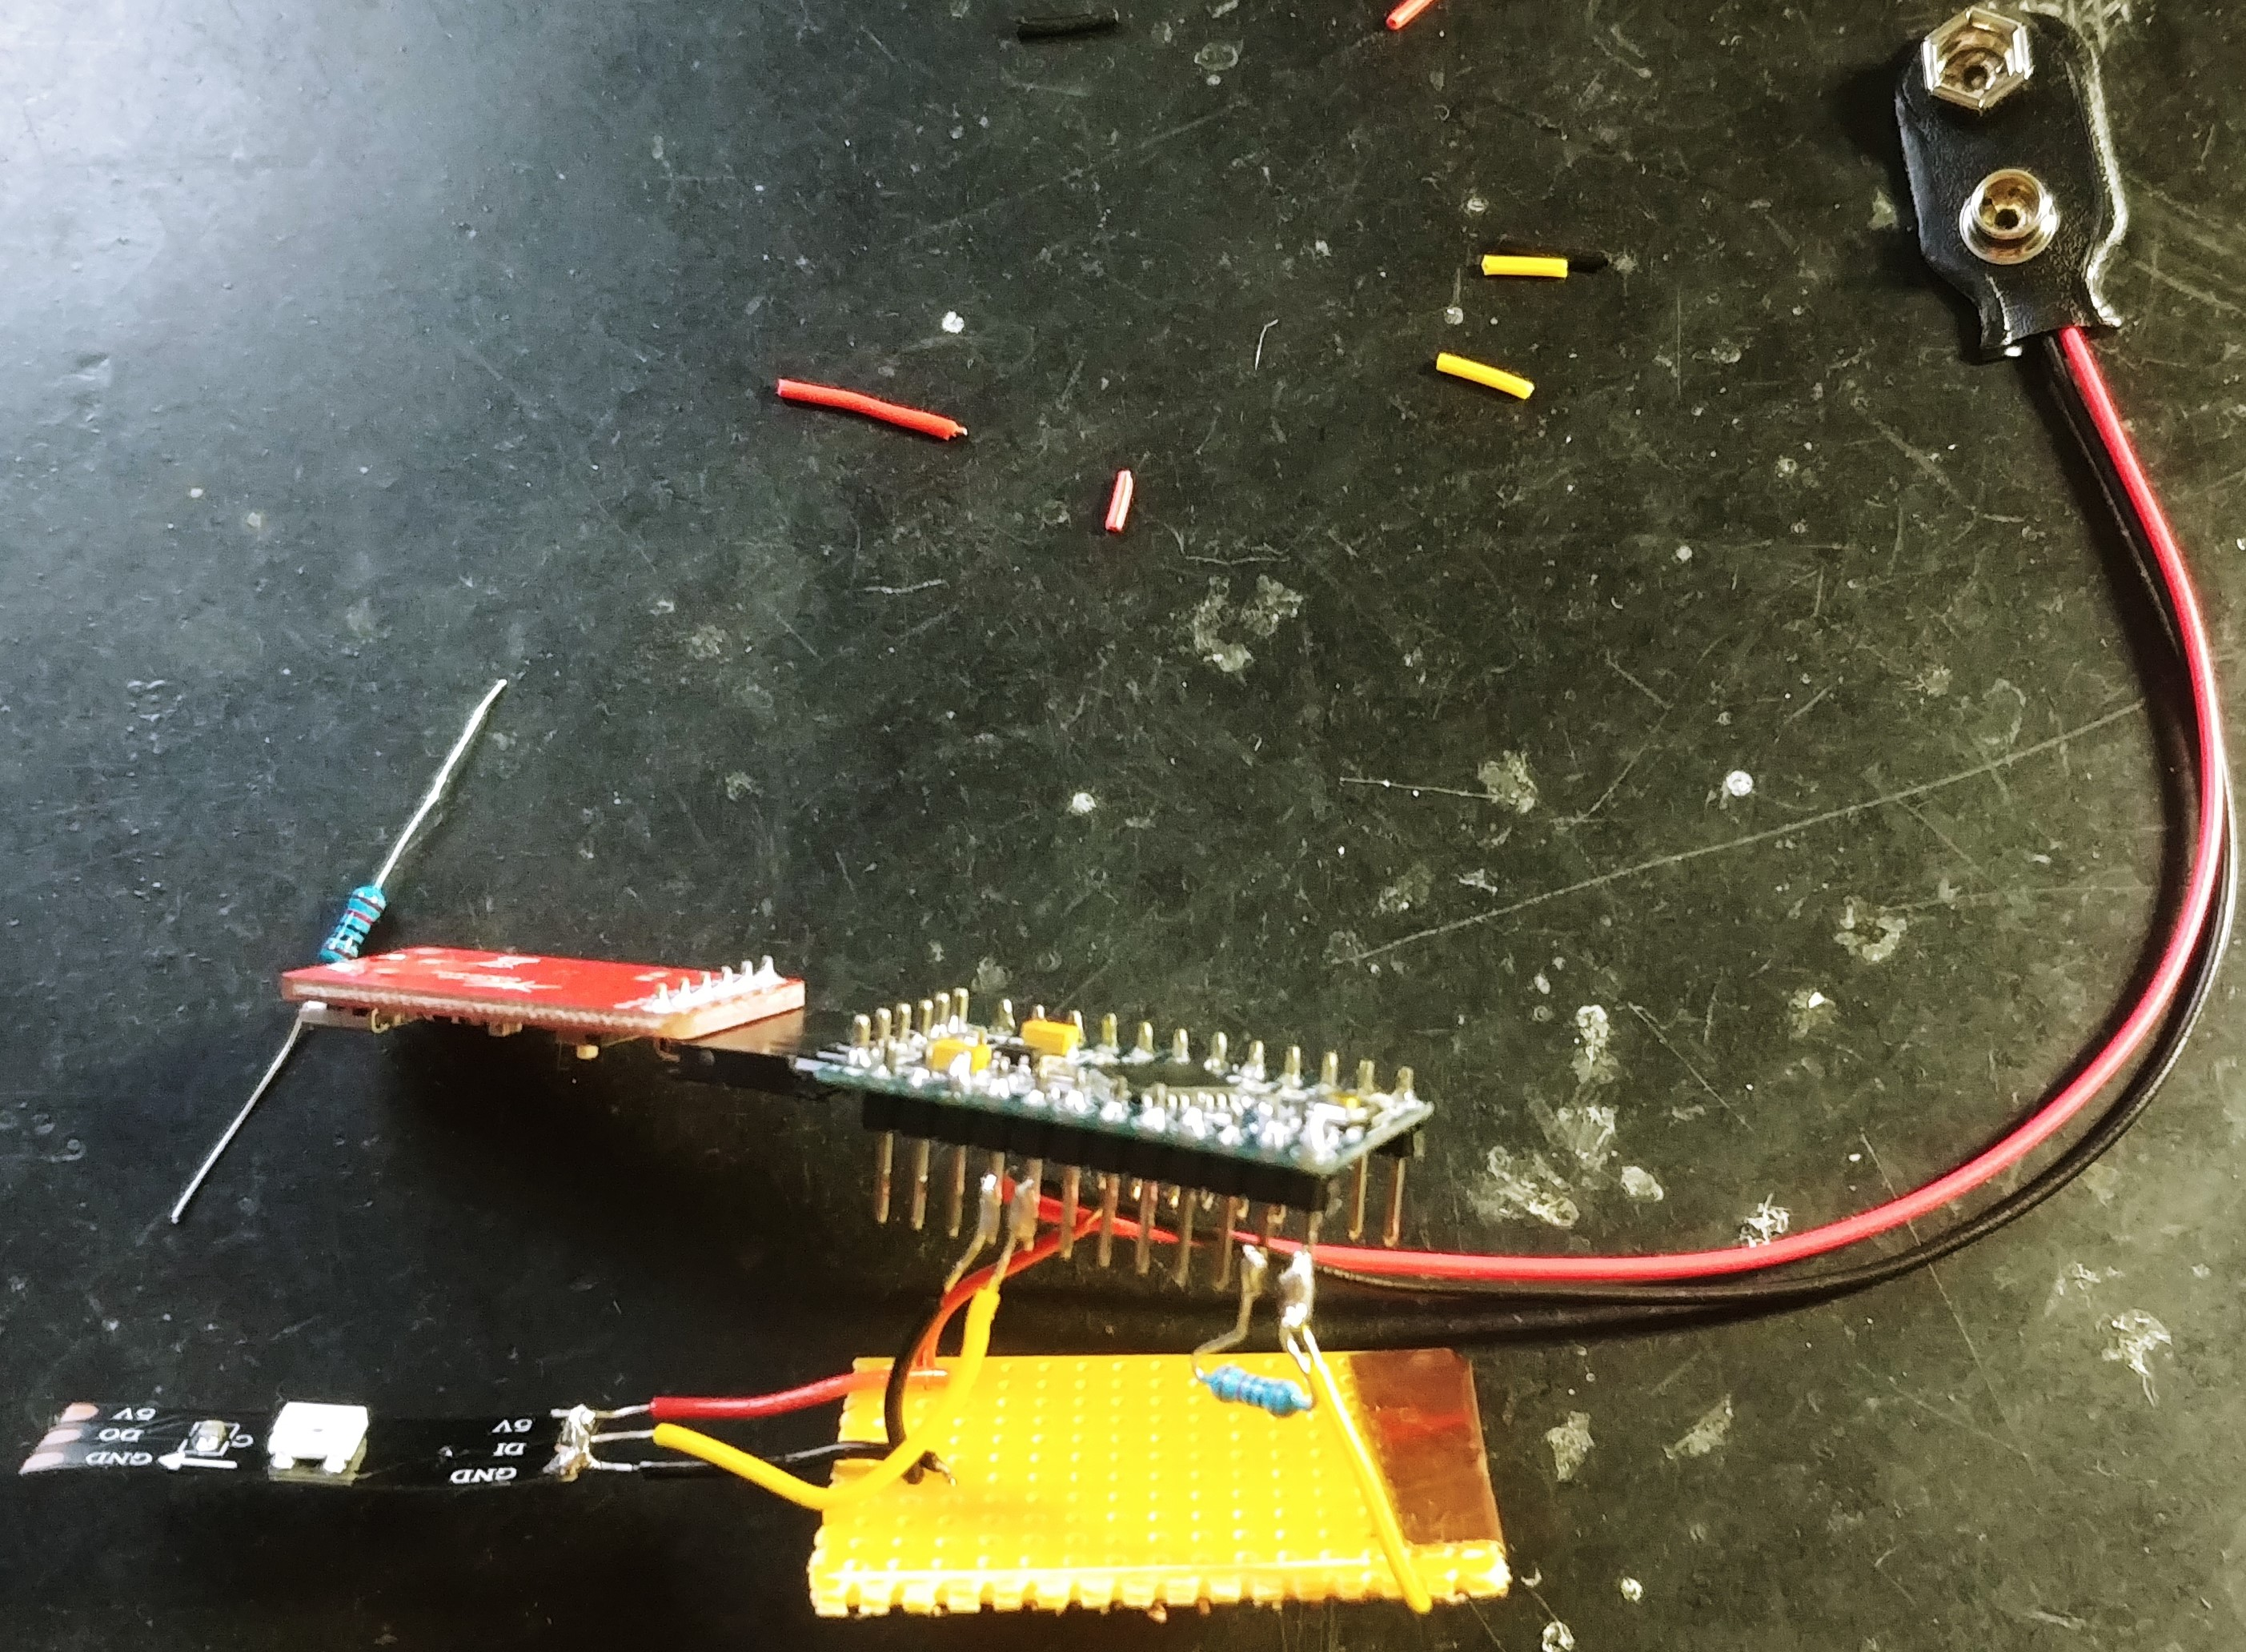
\includegraphics[width=0.8\linewidth]{images/process/solderingProcess.jpg}
        \caption{Shows a testing soldering.}
        \label{fig:solderingProcess_0}
        \vspace{6mm}
        \end{subfigure}
        \begin{subfigure}{.45\textwidth}
            \centering
            \includegraphics[scale=0.03]{images/process/Soldering_Process_1.jpg}
            \caption{Shows the soldering process from the top.}
            \label{fig:solderingProcess_1}
            \vspace{6mm}
        \end{subfigure}
        \hspace{1mm}
        \begin{subfigure}{.45\textwidth}
            \centering
            \includegraphics[scale=0.03]{images/process/Soldering_Process_2.jpg}
            \caption{Shows the soldering process from the botton.}
            \label{fig:solderingProcess_2}
            \vspace{6mm}
        \end{subfigure}
        \begin{subfigure}{.45\textwidth}
            \centering
            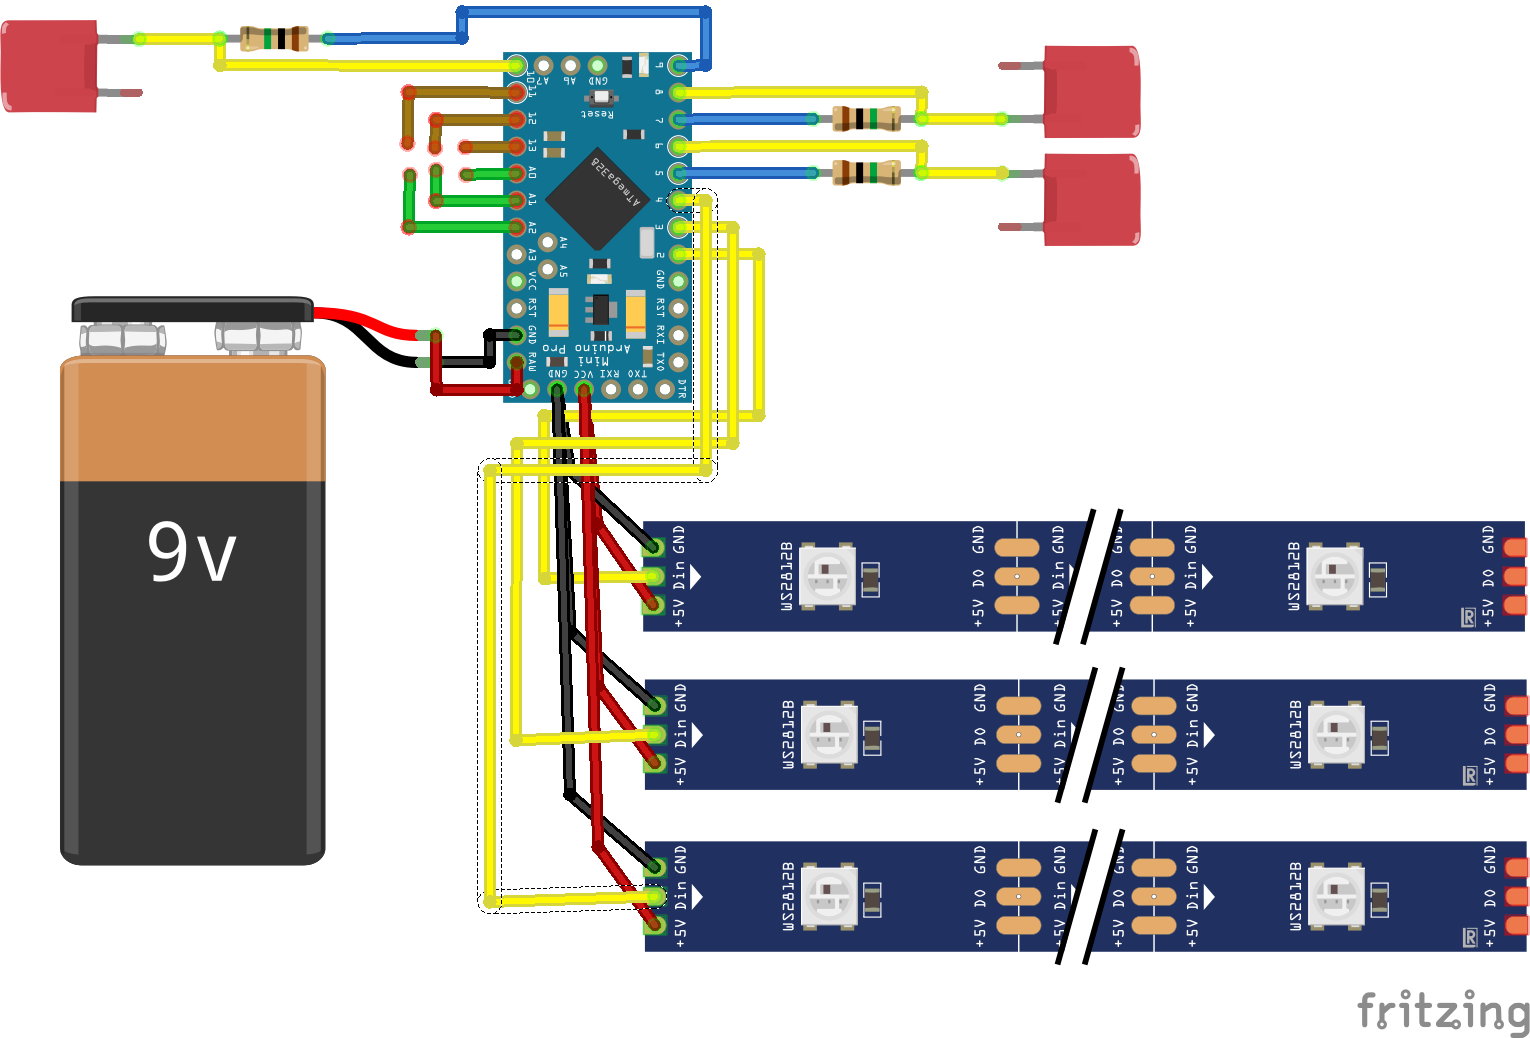
\includegraphics[width=0.8\linewidth]{images/process/sensorLinks.png}
            \caption{Shows the links between the microcontroller and the LEDs and copper foil that is 
            used as a capacitive sensor. This image has been done by Frizing. \cite{fritzing}}
            \label{fig:solderingProcess_3}
            \vspace{6mm}
        \end{subfigure}
        \caption{Shows the soldering process and linking.}
        \label{fig:solderingProcess}
    \end{figure}

    \noindent
    To program these functionalities, we programmed an Arduino program that can deal with these inputs 
    and outputs. The final code can be found on GitHub. %TODO: Add right webpage

\end{document}
